%!TEX root=masterproef.tex

\subsection{Reputatie en vertrouwen}
\label{subsection:reputation}

De probleemstelling dat knopen in het netwerk elkaar niet langer kunnen
vertrouwen, zette verschillende onderzoekers aan tot het zoeken naar
oplossingen gebaseerd op reputatie en vertrouwen.

\citep{ganeriwal2008reputation} beschrijft een architectuur gebaseerd op
observaties door knopen van de acties van andere knopen in het kader van acties
van zichzelf of derde knopen. Figuur \ref{fig:reputation-cooperation} toont de
situaties die beschouwd worden: in \ref{fig:reputation-cooperative-node} zal
een co\"operatieve knoop (C) alle boodschappen die via hem verzonden worden
door een zendende knoop (Z) effectief doorsturen naar een verder gelegen
ontvangende knoop (O). De verzender van de boodschap, alsook andere naburige
knopen (B) kunnen deze actie vaststellen. In
\ref{fig:reputation-uncooperative-node} daarentegen zal een een
niet-co\"operatieve knoop (NC) deze boodschappen niet verder versturen of zelfs
aanpassen.

\begin{figure}
\centering
\begin{subfigure}{.49\textwidth}
\centering
  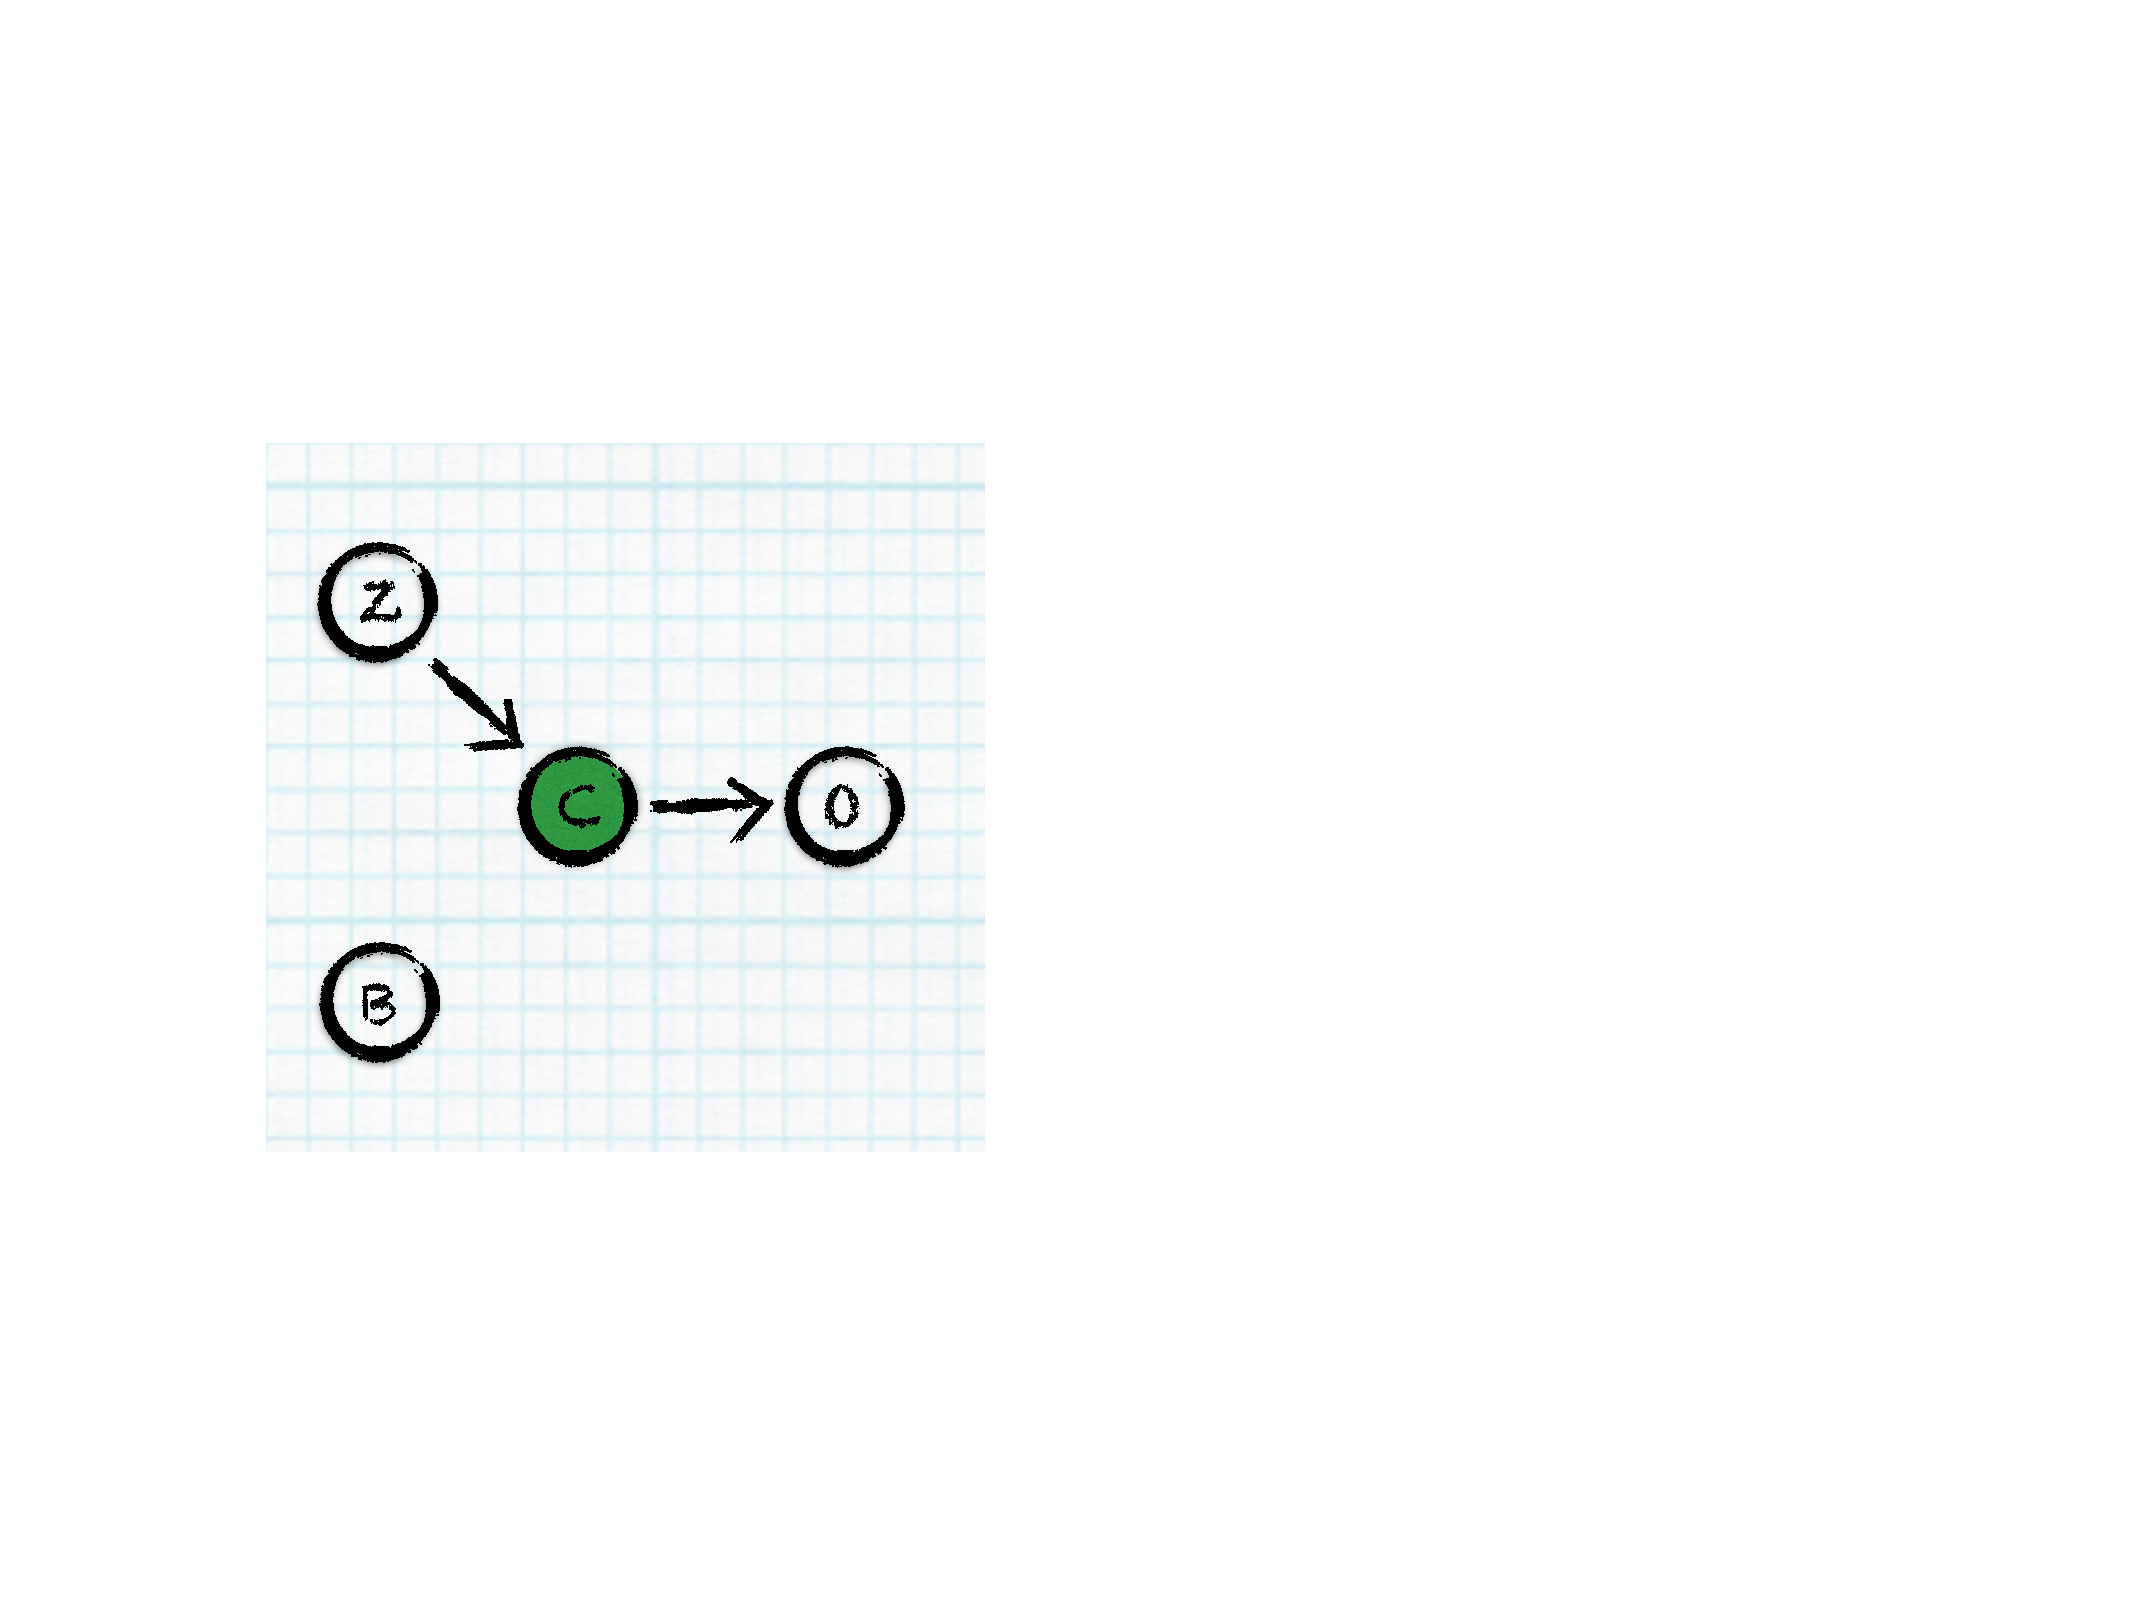
\includegraphics[width=.8\linewidth]{./resources/cooperative.pdf}
  \caption{Co\"operatieve knoop}
  \label{fig:reputation-cooperative-node}
\end{subfigure}
\begin{subfigure}{.49\textwidth}
\centering
  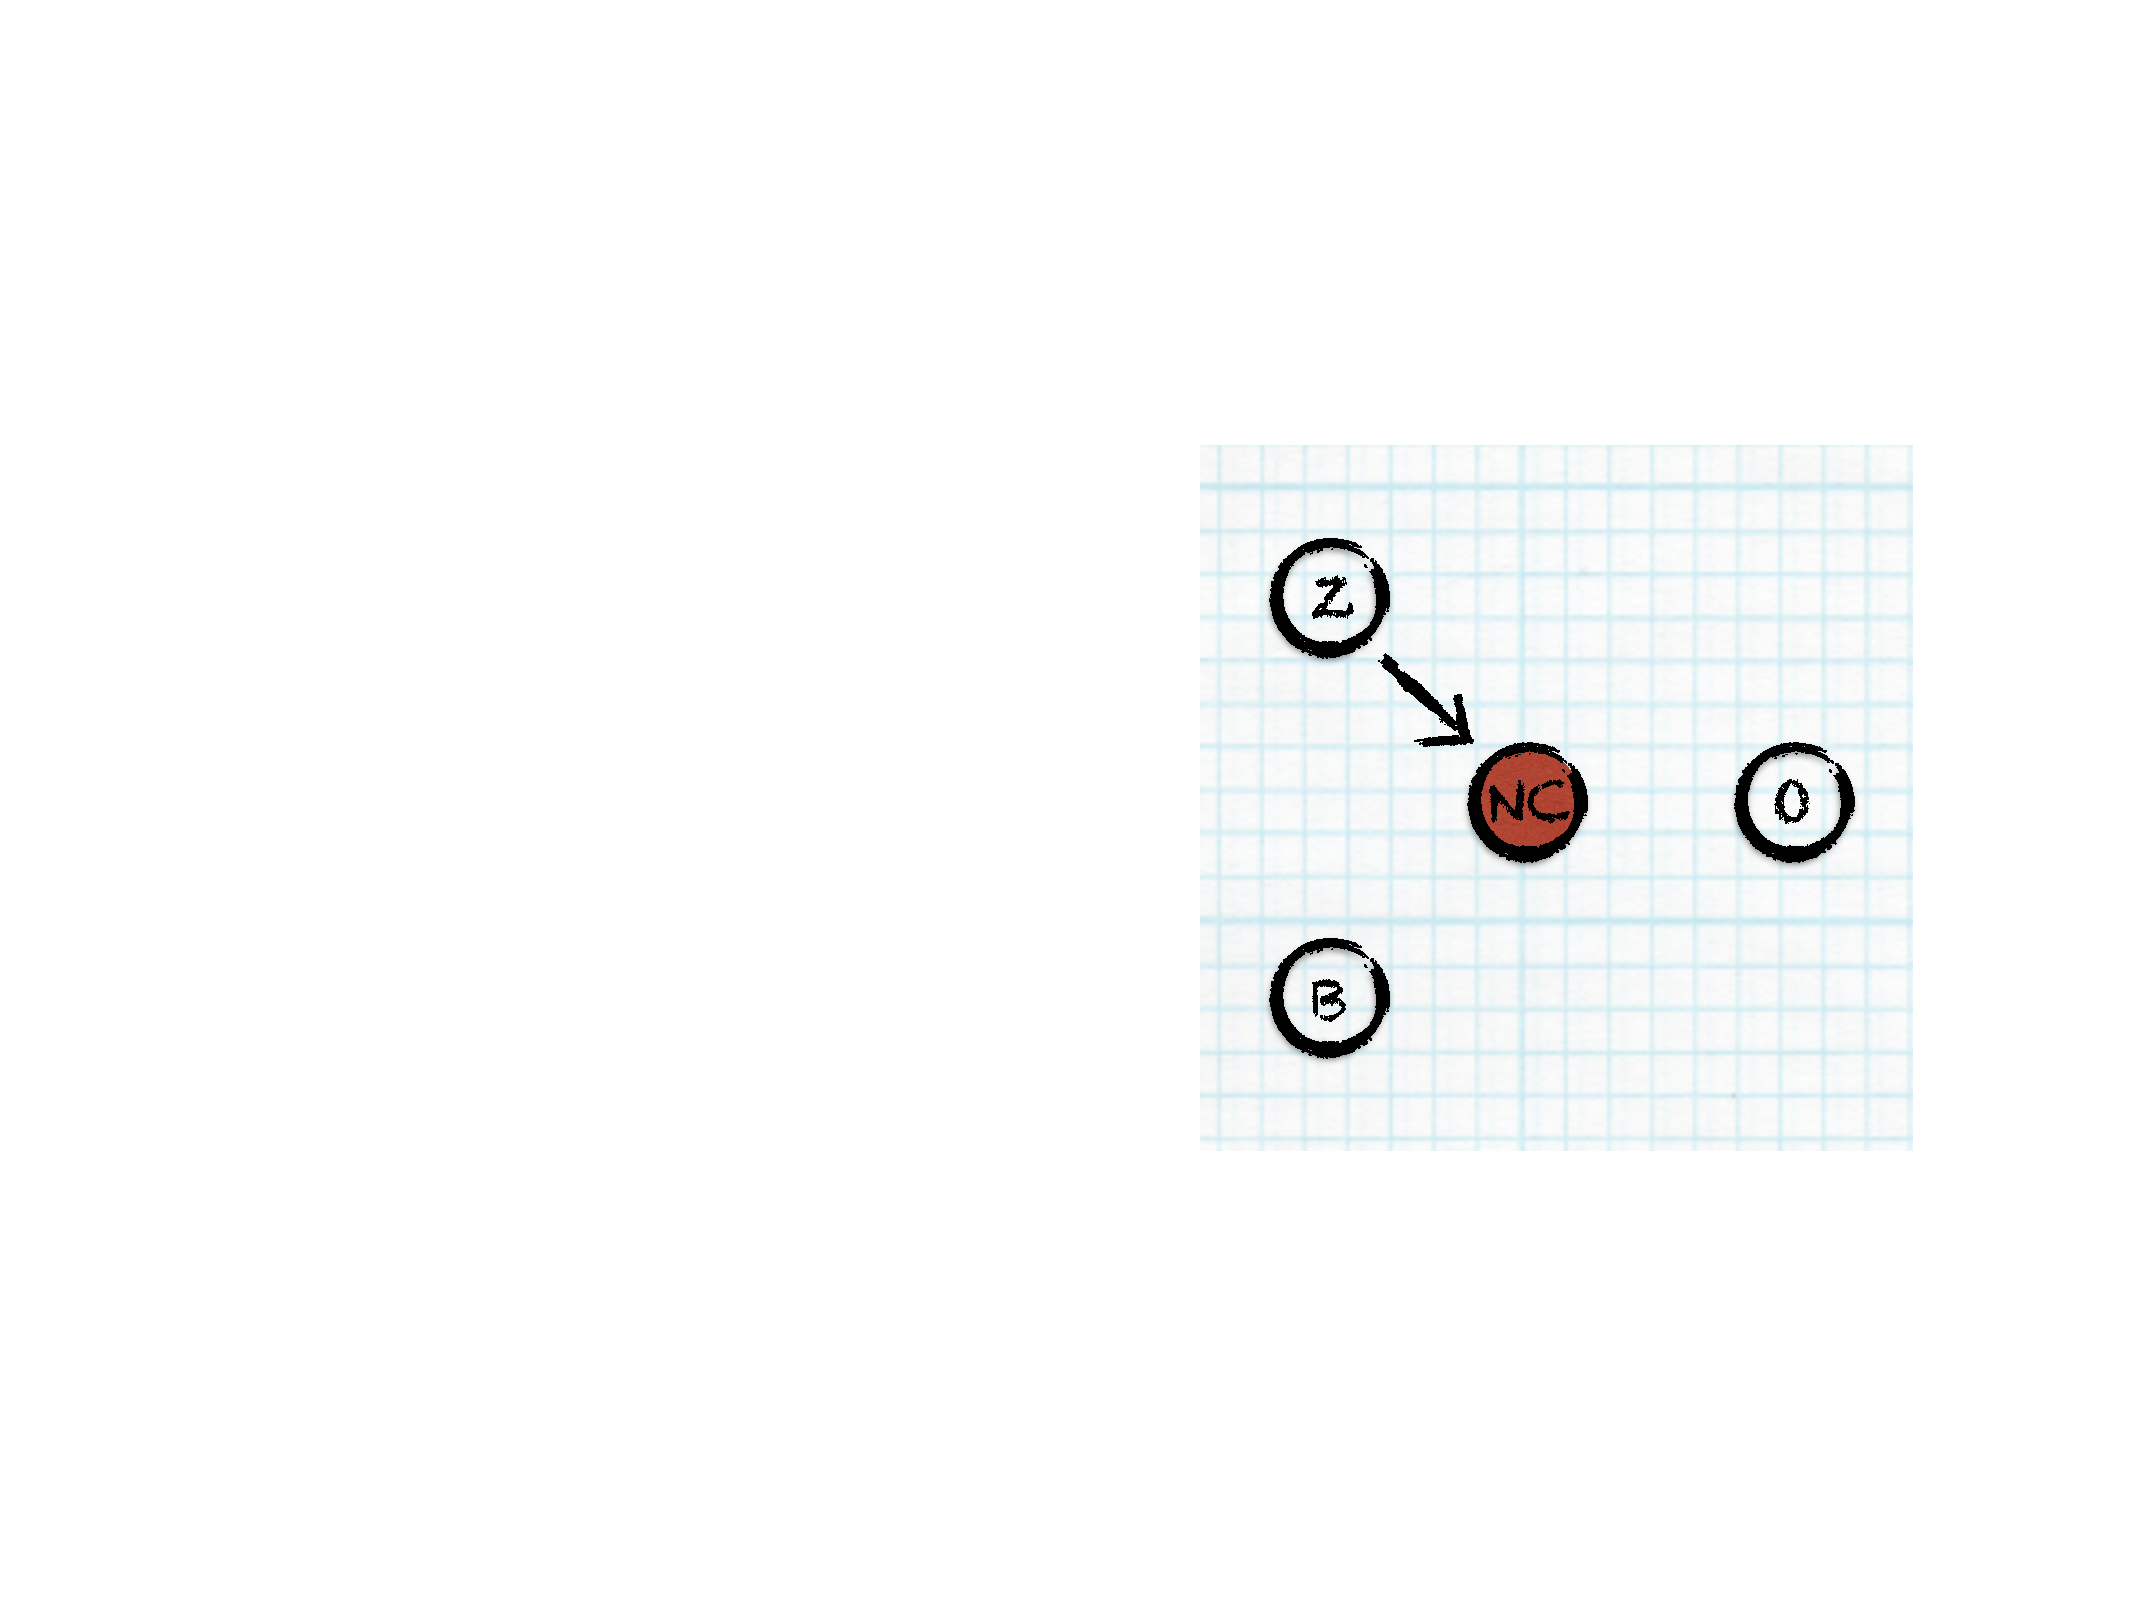
\includegraphics[width=.8\linewidth]{./resources/non-cooperative.pdf}
  \caption{Niet-co\"operatieve knoop}
  \label{fig:reputation-uncooperative-node}
\end{subfigure}
\caption{Beschouwde situaties bij al dan niet co\"operatieve knopen.}
\label{fig:reputation-cooperation}
\end{figure}

Op basis van deze situatie stellen de auteurs dat reputatie van een knoop kan
weergegeven worden aan de hand van een beta distributie. Bijlage
\ref{appendix:reputation} bespreekt de mathematische onderbouw.

De auteurs vermelden zelf een zeer belangrijk probleem: omdat knopen constant
moeten luisteren naar de acties van naburige knopen, moeten zij constant actief
zijn. Dit is een zeer nadelig uitgangspunt voor systemen die typisch trachten
zuinig om te springen met hun energie.

Maar de architectuur heeft ook inherente problemen en laat kwaadwillige
partijen toe om - mits kennis van de parameters - net onder de radar te
opereren. We illustreren dit met de simulatie zoals deze uitgevoerd werd door
de auteurs.

De evolutie van een volledige co\"operatieve of volledige niet-co\"operatieve
knoop wordt weergegeven in figuur \ref{fig:reputation-paper}. Een eigenschap
van het algoritme is dat pas na een tiental (louter positieve) observaties een
knoop de drempelwaarde van vertrouwen overschrijdt.

\begin{figure}[ht]
\centering
\begin{subfigure}{.49\textwidth}
  \centering
  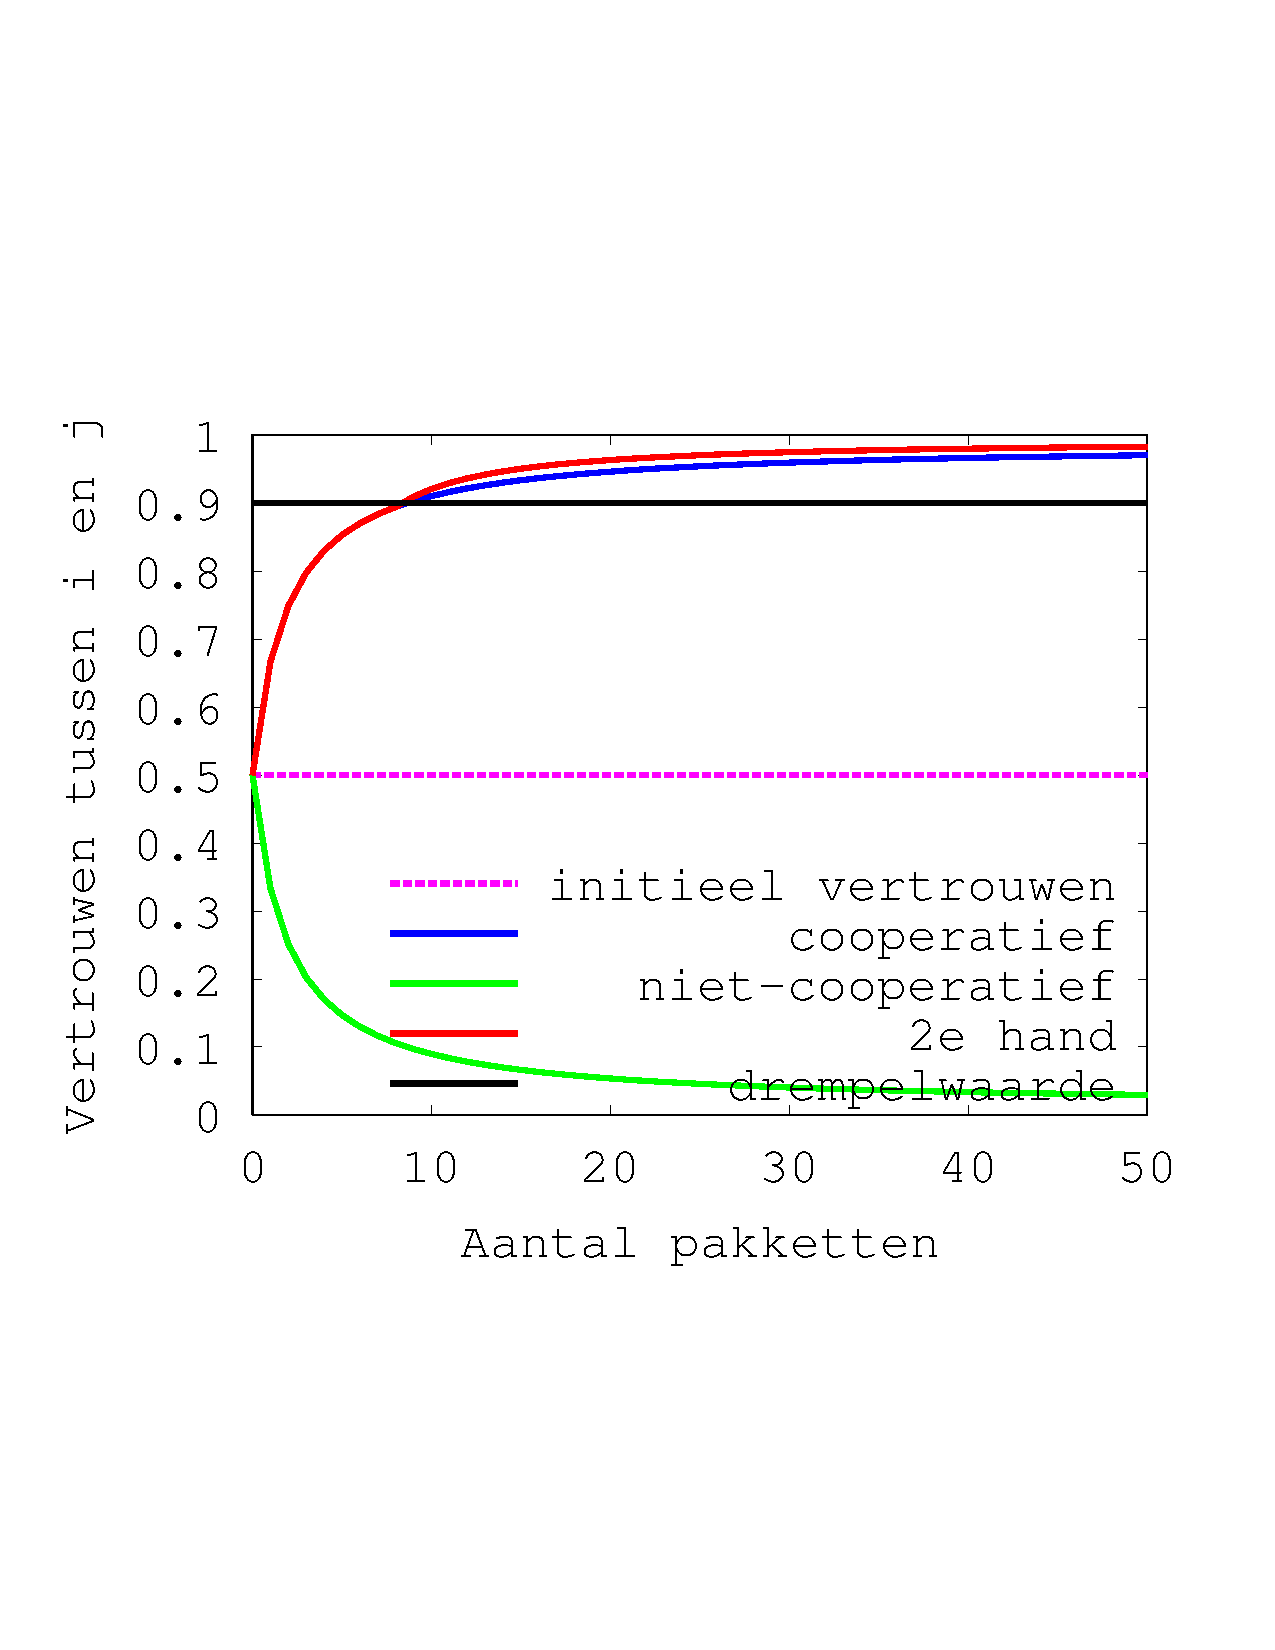
\includegraphics[width=.9\linewidth]{./resources/reputation-paper.pdf}
  \caption{Co\"operatieve en niet-co\"operatieve knopen}
  \label{fig:reputation-paper}
\end{subfigure}
\begin{subfigure}{.49\textwidth}
  \centering
  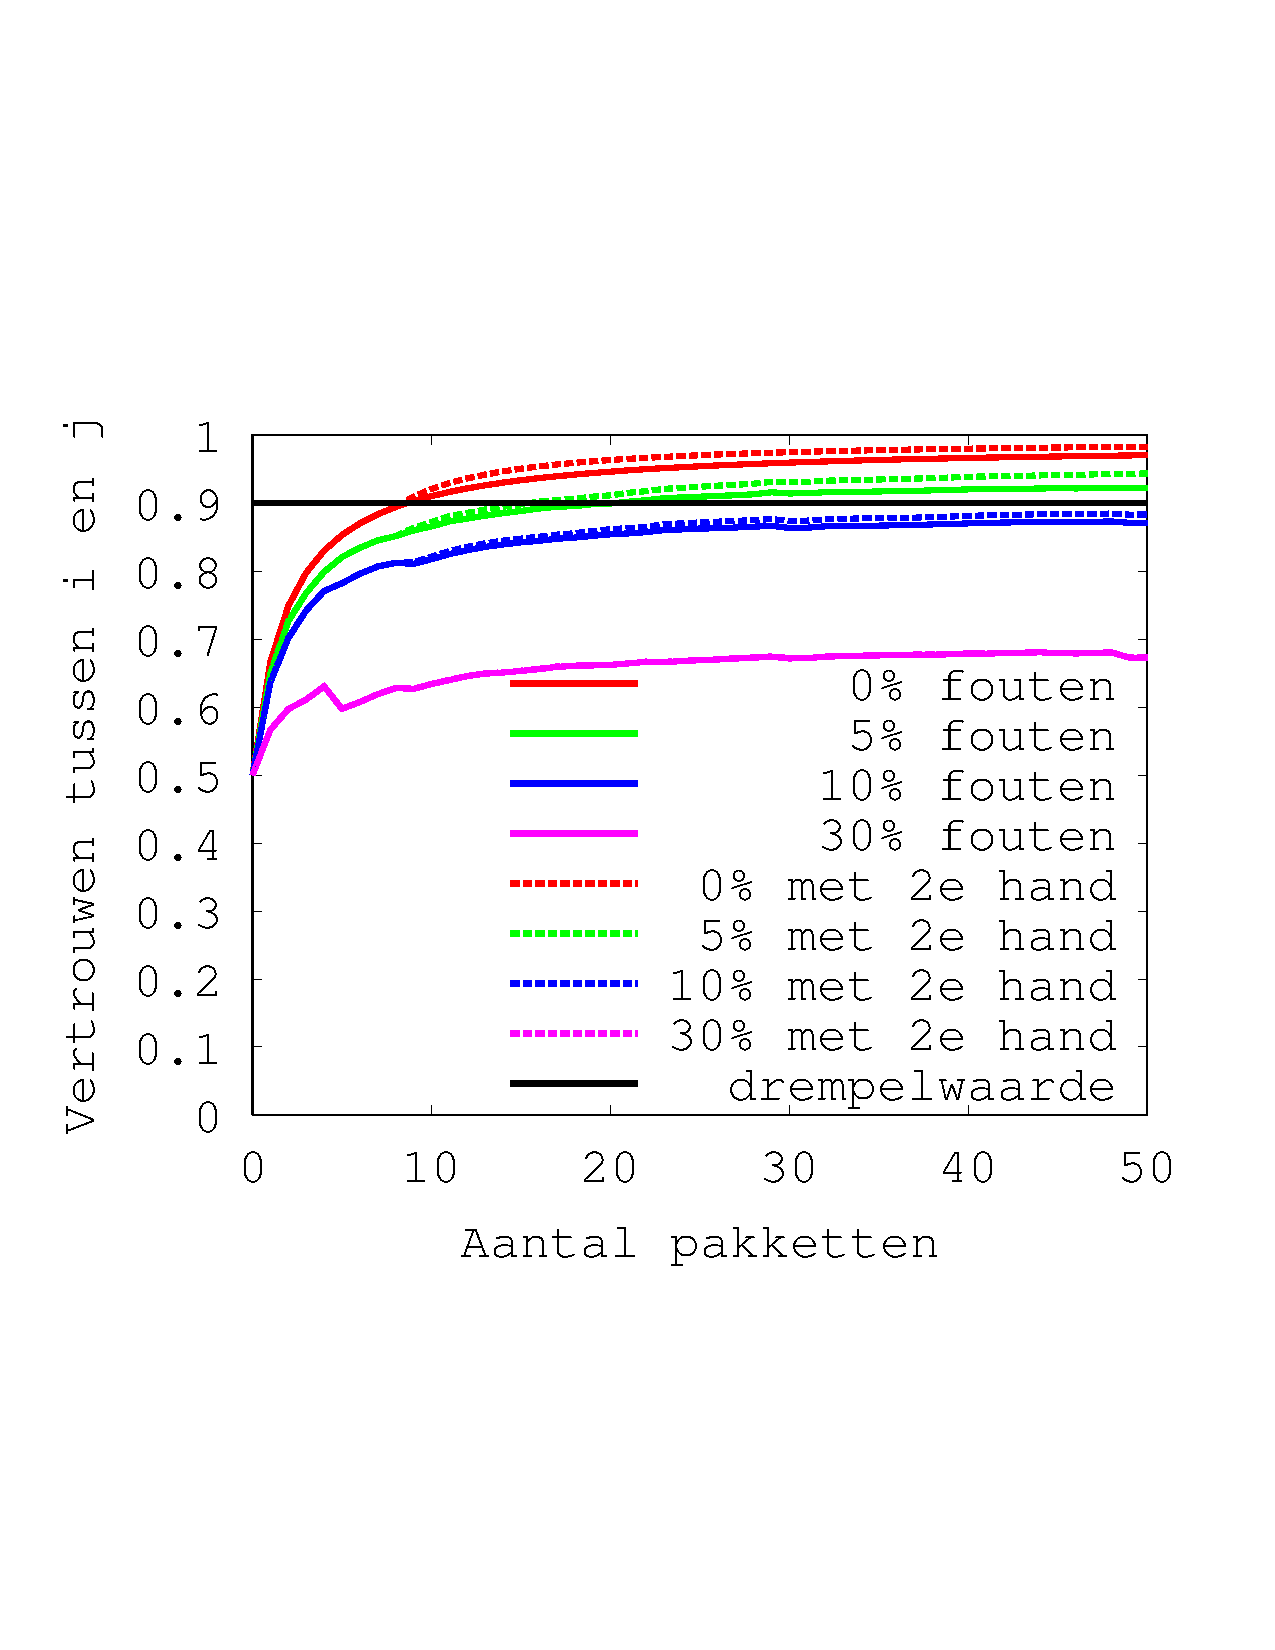
\includegraphics[width=.9\linewidth]{./resources/reputation-with-failure.pdf}
  \caption{Falende knopen (100 simulaties)}
  \label{fig:reputation-with-failure}
\end{subfigure}
\caption{Impact van falende knopen op evolutie van vertrouwen.}
\label{fig:reputation-paper-with-failure}
\end{figure}

Deze eigenschap kan echter misbruikt worden zoals aangetoond wordt in figuur
\ref{fig:reputation-with-failure}. Stel dat een knoop $j$ te kampen heeft met
falende hardware, waardoor 5\% van zijn transmissies verloren gaan en daarom
ook niet opgemerkt kunnen worden door andere knopen.

We merken op dat deze knoop, zelfs met 5\% niet-co\"operatieve observaties, na
een twintigtal observaties toch boven de drempelwaarde uitkomt en door de
beschouwende knoop aanvaard wordt als betrouwbaar.

Vanuit een operationeel standpunt gezien is dit in eerste instantie een
positief effect. Indien een knoop \emph{slechts} 5\% faalt zal deze toch als
co\"operatief beschouwd worden en de goede werking van het netwerk niet
fundamenteel in het gedrang brengen - vanuit een inbraakdetectie oogpunt gezien.

Maar stel dat deze 5\% niet-co\"operatieve acties geen falen zijn en dat de
doorgestuurde boodschappen niet verloren gaan, maar met opzet lichtjes
gewijzigd worden. 5\% kan een significante vertekening van metingen van een
netwerk betekenen en zo de werking van het hele netwerk ondermijnen.

Figuur \ref{fig:reputation-malicious} gaat slechts een kleine stap verder en
toont het effect van falende (of malafide) knopen die pas falingen vertonen
nadat ze het vertrouwen hebben gekregen van een knoop. We merken op dat nu zelfs
10\% falingen zeer lang het vertrouwen kunnen behouden.

\begin{figure}[ht]
 \centering
 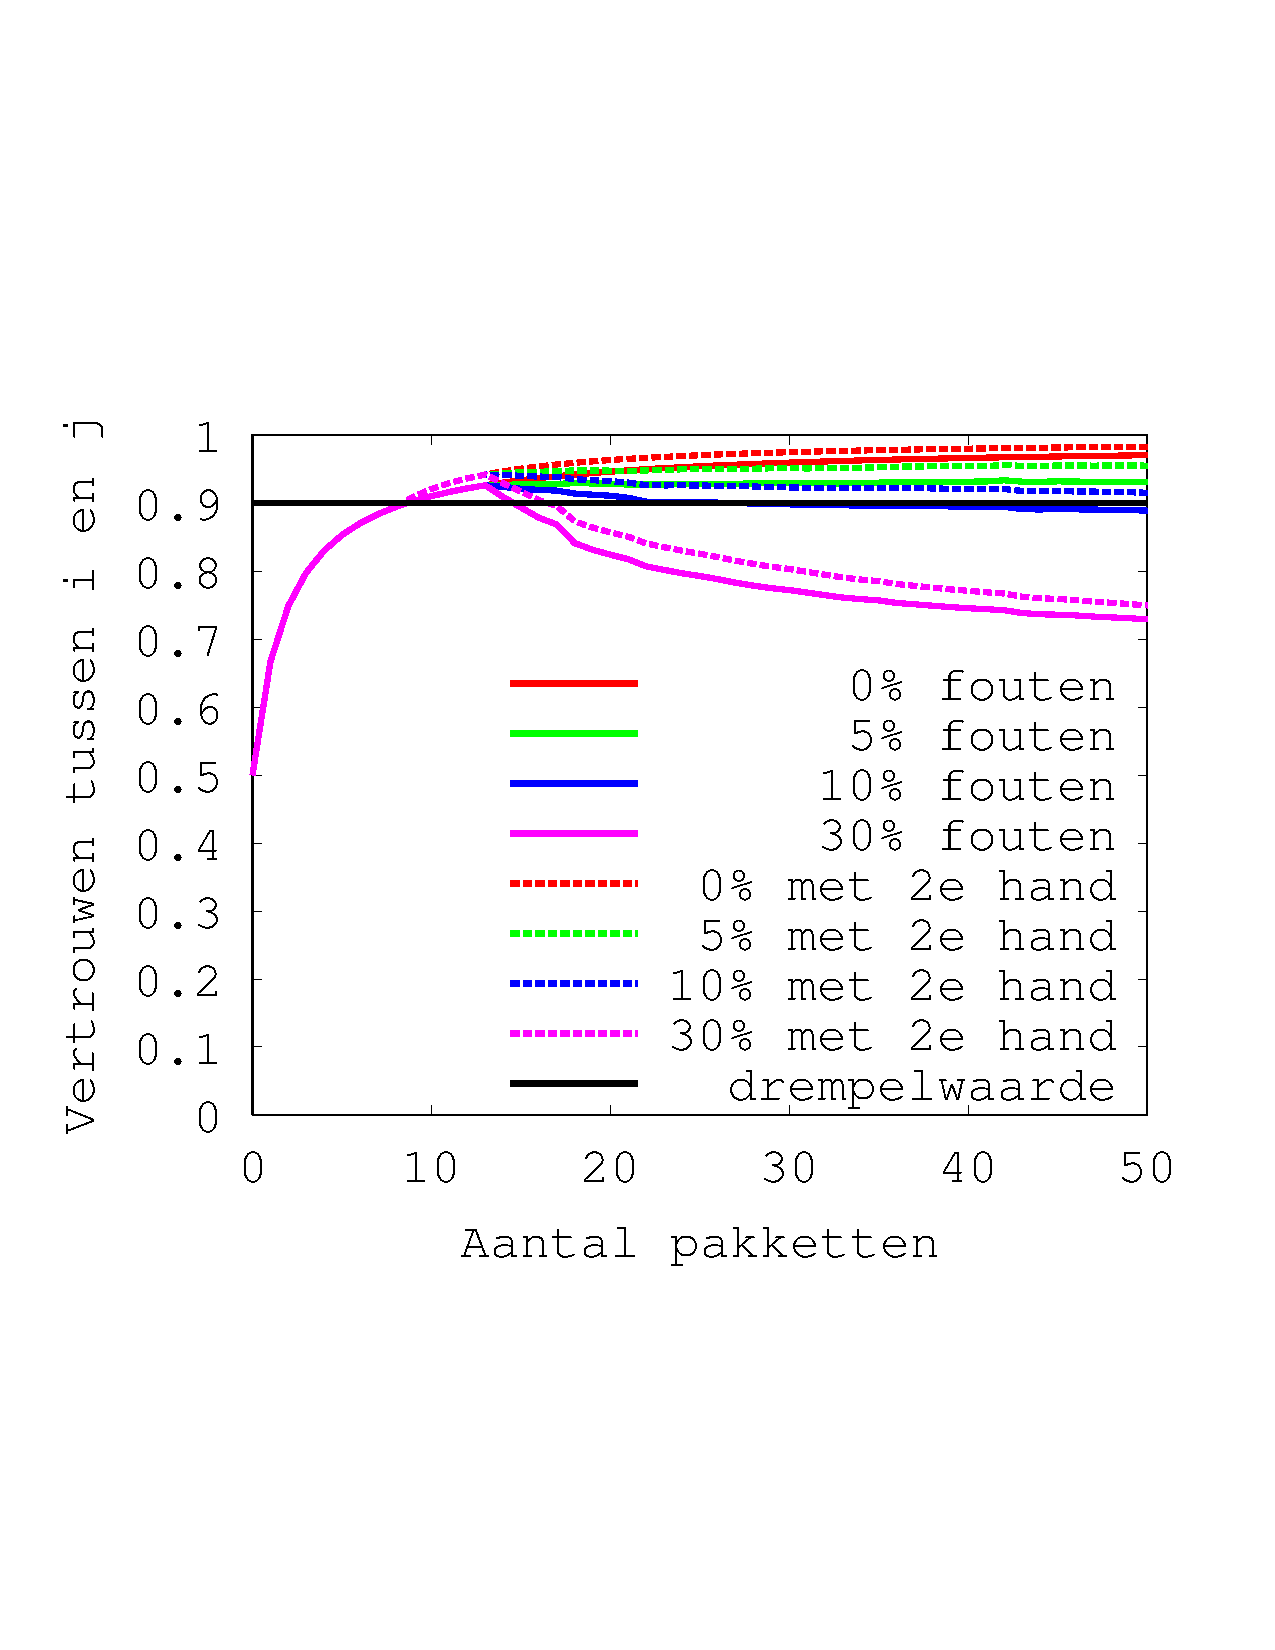
\includegraphics[width=.5\linewidth]{./resources/reputation-malicious.pdf}
 \caption{Falende knopen met vertraging van 15 pakketten (100 simulaties)}
 \label{fig:reputation-malicious}
\end{figure}

Dit elementaire voorbeeld toont duidelijk aan dat het vaststellen van een
reputatie op basis van externe observaties een zeer delicaat onderwerp is dat
zeer gevoelig is voor manipulatie op basis van kennis van de interne
parameters. Dit laatste is dan weer net \'e\'en van d\'e problemen waar
draadloze sensornetwerken mee kampen omdat knopen vrij eenvoudig kunnen
weggenomen, ge\"inspecteerd, gewijzigd en teruggeplaatst worden.
